\documentclass{article}
\usepackage{graphicx}
\usepackage{amsmath}
\usepackage{booktabs}
\usepackage{array}
\usepackage{hyperref}
\usepackage{float}
\usepackage{tikz}
\usepackage{circuitikz}
\usepackage{karnaugh-map}
\usepackage{subcaption}

\title{\textbf{Lab Report: Experiment 9}}
\author{EE24BTECH11003 : Akshara Sarma Chennubhatla\\EE24BTECH11005 : Arjun Pavanje}

\begin{document}
\maketitle
\begin{center}
	\textbf{Experiment:}\\Designing a Moore Finite State Machine\\to detect the sequence 11011\\in the case of overlapping signals\\using T flip-flops and logical gates
\end{center}
\vspace{30pt}
\begin{figure}[h!]
	\centering
	
\includegraphics[width = 100pt]{.logo/logo.png}\\
\end{figure}
\begin{center}
	Bachelor of Technology\\
	\vspace{10pt}
	Department of Electrical Engineering\\
\end{center}
\newpage
\section{Objective}
Design and implement a Moore finite state machine (FSM) to detect the sequence \textbf{11011}. The output should be \textbf{1} (LED glows) only when this sequence is detected.

\section{Materials Required:}

\begin{itemize}
    \item LED
    
    \item JK (or T) flipflops
    
    \item AND Gates 
    
    \item OR Gates
    
    \item Breadboard \& Jumper Wires
    
    \item Arduio UNO (or some other microcontroller)
    
\end{itemize}

\section{Circuit}
\begin{figure}[h!]
    \centering
    %\rotatebox{90}{
    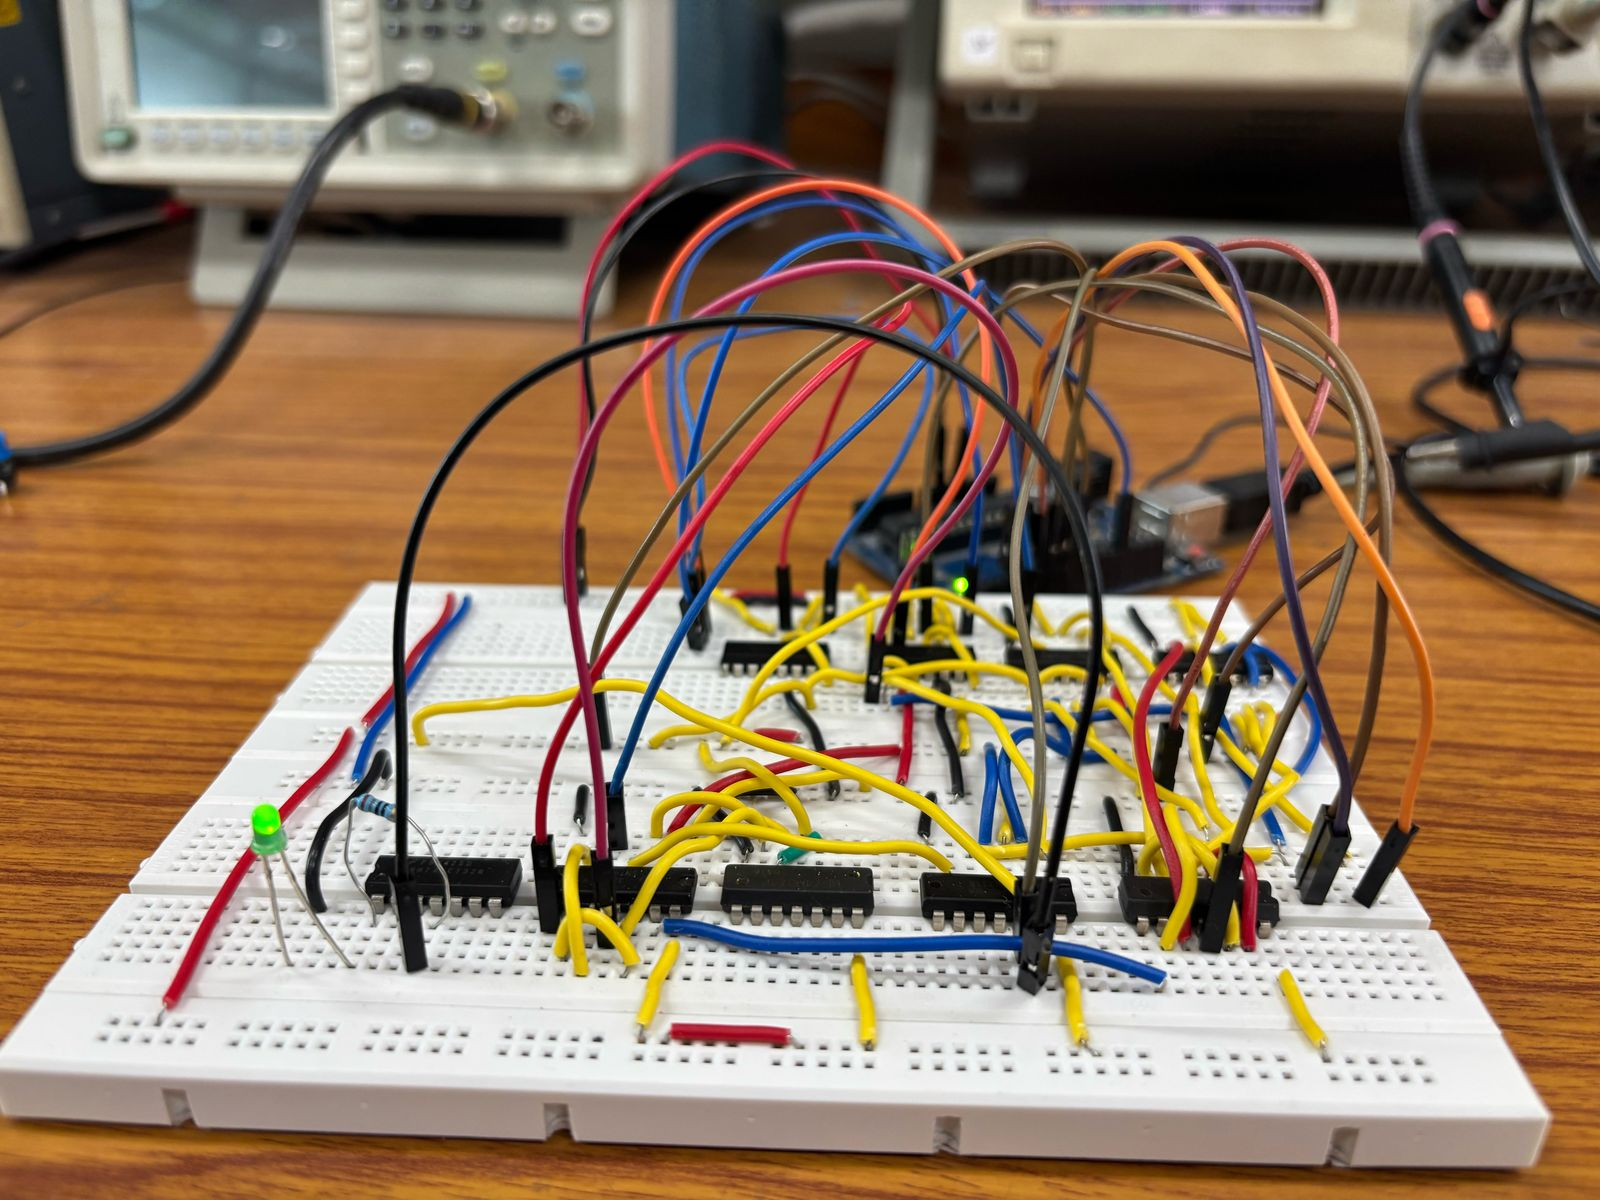
\includegraphics[width=0.7\linewidth]{figs/circuit.png}
    \caption{Circuit}
    \label{fig:enter-label}
\end{figure}
The circuit may look daunting and complicated at first, let us break it down and study each module seperately.
\pagebreak
\subsection{Overview}
\begin{figure}[h!]
    \centering
    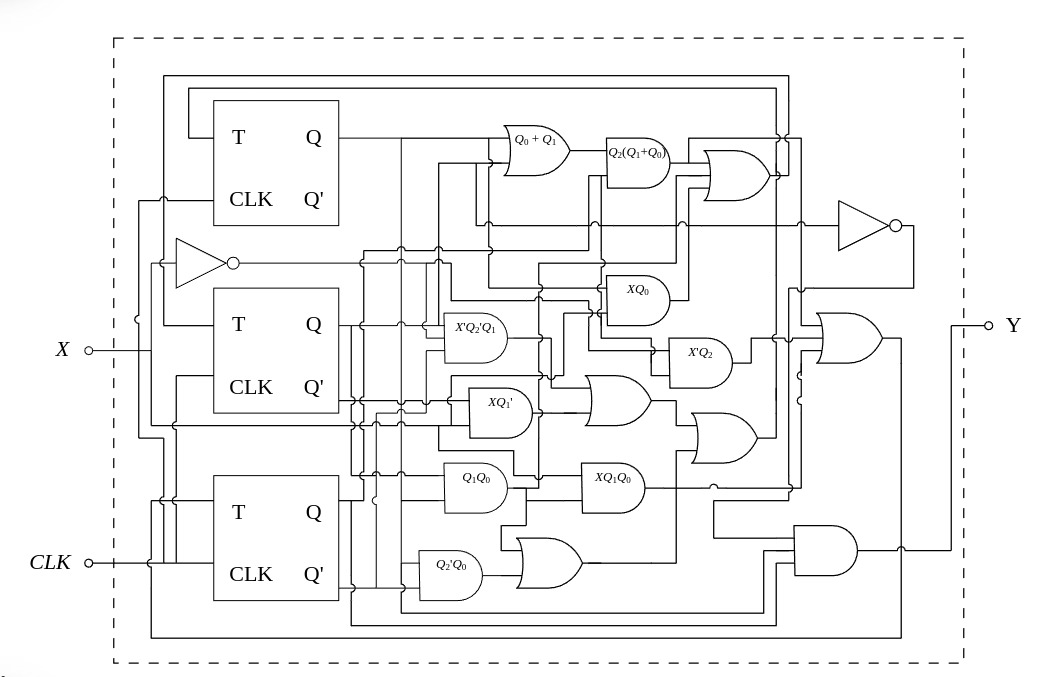
\includegraphics[width=1\linewidth]{figs/overview.png}
    \caption{Circuit Overview}
    \label{fig:enter-label}
\end{figure}

\subsection{JK to T Flip-Flop Conversion}
Since JK flip-flops were provided instead of T flip-flops, conversion was necessary. Converting a JK flip-flop to a T flip-flop can be done by simply shorting J and K ports of JK flip-flops.
\begin{displaymath}
\begin{array}{|c| c|c|c |c|}
\hline
T & Q_n & Q_{n+1} & J & K \\
\hline
0 & 0 & 0 & 0 & X \\
0 & 1 & 1 & X & 0 \\
1 & 0 & 1 & 1 & X \\
1 & 1 & 0 & X & 1 \\
\hline
\end{array}
\end{displaymath}
Writing Karnaugh-map for $J$
\begin{center}
\begin{karnaugh-map}[2][2][1][$Q_n$][$T$]
    \manualterms{0,X,1,X}
    \implicant{2}{3}
    %\implicant{5}{15}
    %\implicantedge{1}{3}{9}{11}
    %\implicantcorner
    %\implicantedge{4}{12}{6}{14}
\end{karnaugh-map}
\end{center}
We get,
\begin{align*}
    J = T
\end{align*}
Now writing karnaugh-map for $K$,
\begin{center}
\begin{karnaugh-map}[2][2][1][$Q_n$][$T$]
    \manualterms{X,0,X,1}
    \implicant{2}{3}
    %\implicant{5}{15}
    %\implicantedge{1}{3}{9}{11}
    %\implicantcorner
    %\implicantedge{4}{12}{6}{14}
\end{karnaugh-map}
\end{center}
We get,
\begin{align*}
    K = T
\end{align*}
\pagebreak
\subsection{State Diagram}

\begin{figure}[!ht]
\centering
\resizebox{1\textwidth}{!}{%
\begin{circuitikz}
\tikzstyle{every node}=[font=\LARGE]
\draw (8.5,21.5) to[short] (8.5,21.5);
\draw  (11.25,15.75) circle (1.25cm);
\draw  (17.25,12.5) circle (1.25cm);
\draw  (17.75,6.25) circle (1.25cm);
\draw  (11.25,2.5) circle (1.25cm);
\draw  (5,6.5) circle (1.25cm);
\draw  (5.25,12.25) circle (1.25cm);
\draw [->, >=Stealth] (12.5,15.75) .. controls (13.5,15.75) and (15.25,14.75) .. (16.5,13.5) ;
\draw [->, >=Stealth] (17.75,11.25) .. controls (18.25,10) and (18.5,8.5) .. (18,7.5) ;
\draw [->, >=Stealth] (17,5.25) .. controls (15.75,3.25) and (14.25,2.75) .. (12.5,2.25) ;
\draw [->, >=Stealth] (10,2.25) .. controls (8,2.5) and (6.25,3.5) .. (5.25,5.25) ;
\draw [->, >=Stealth] (4.5,7.75) .. controls (4.25,8.75) and (4.25,10) .. (4.75,11) ;
\node [font=\LARGE] at (11.5,15.75) {$S_0$};
\node [font=\LARGE] at (17.25,12.5) {$S_1$};
\node [font=\LARGE] at (17.75,6.25) {$S_2$};
\node [font=\LARGE] at (11.25,2.5) {$S_3$};
\node [font=\LARGE] at (5,6.5) {$S_4$};
\node [font=\LARGE] at (5.25,12.25) {$S_5$};
\node [font=\LARGE] at (14.25,14.25) {1/0};
\node [font=\LARGE] at (19,9.75) {1/0};
\node [font=\LARGE] at (16.25,3) {0/0};
\node [font=\LARGE] at (6.5,2.75) {1/0};
\node [font=\LARGE] at (5,8.75) {1/0};
\draw [->, >=Stealth] (5.5,11) .. controls (5.75,8.75) and (7.5,4.25) .. (10.75,3.75) ;
\draw [->, >=Stealth] (6.25,11.5) .. controls (8.25,8.75) and (11.5,6.25) .. (16.5,6.5) ;
\node [font=\LARGE] at (8,6.75) {0/1};
\node [font=\LARGE] at (11.5,8.25) {1/1};
\draw [->, >=Stealth] (10.75,17) .. controls (10.25,19.5) and (12.25,19) .. (11.5,17) ;
\draw [->, >=Stealth] (18.5,12.75) .. controls (19.5,17.25) and (13,18.75) .. (12,16.75) ;
\draw [->, >=Stealth] (19,6.5) .. controls (21.25,6) and (20,4.75) .. (18.75,5.5) ;
\draw [->, >=Stealth] (11.5,3.75) .. controls (9.5,4.5) and (8.5,12.25) .. (11,14.5) ;
\draw [->, >=Stealth] (4,7.25) .. controls (1.75,13.25) and (4.75,15.5) .. (10,16) ;
\node [font=\LARGE] at (9,12) {0/0};
\node [font=\LARGE] at (3.5,14.25) {0/0};
\node [font=\LARGE] at (11,19.25) {0/0};
\node [font=\LARGE] at (20.75,5.25) {1/0};
\node [font=\LARGE] at (17.5,17.25) {0/0};
\end{circuitikz}
}%

\label{fig:my_label}
\end{figure}
\pagebreak

\subsection{Transition Table}

\begin{center}
\begin{tabular}{|c|c|c|c|c|c|c|c|c|c|c|}
%\begin{tabular}{|c|c|c|c|c|c|c|c|c|}
\hline
$Q_2$ & $Q_1$ & $Q_0$ & $X$ & $T_2$ & $T_1$ & $T_0$ & $Q_2'$ & $Q_1'$ & $Q_0'$ & $Y$ \\
\hline
0 & 0 & 0 & 0 & 0 & 0 & 0 & 0 & 0 & 0 & 0 \\
0 & 0 & 0 & 1 & 0 & 0 & 1 & 0 & 0 & 1 & 0 \\
0 & 0 & 1 & 0 & 0 & 0 & 1 & 0 & 0 & 0 & 0 \\
0 & 0 & 1 & 1 & 0 & 1 & 1 & 0 & 1 & 0 & 0 \\
0 & 1 & 0 & 0 & 0 & 0 & 1 & 0 & 1 & 1 & 0 \\
0 & 1 & 0 & 1 & 0 & 0 & 0 & 0 & 1 & 0 & 0 \\
0 & 1 & 1 & 0 & 0 & 1 & 1 & 0 & 0 & 0 & 0 \\
0 & 1 & 1 & 1 & 1 & 1 & 1 & 1 & 0 & 0 & 0 \\
1 & 0 & 0 & 0 & 1 & 0 & 0 & 0 & 0 & 0 & 0 \\
1 & 0 & 0 & 1 & 0 & 0 & 1 & 1 & 0 & 1 & 1 \\
1 & 0 & 1 & 0 & 1 & 1 & 0 & 0 & 1 & 1 & 0 \\
1 & 0 & 1 & 1 & 1 & 1 & 1 & 0 & 1 & 0 & 0 \\
1 & 1 & 0 & 0 & 1 & 1 & 0 & 0 & 0 & 0 & 0 \\
1 & 1 & 0 & 1 & 1 & 1 & 0 & 0 & 0 & 0 & 0 \\
1 & 1 & 1 & 0 & 1 & 1 & 1 & 0 & 0 & 0 & 0 \\
1 & 1 & 1 & 1 & 1 & 1 & 1 & 0 & 0 & 0 & 0 \\
\hline
\end{tabular}
\end{center}

\subsection{K-Maps}

% Karnaugh map for T0
\begin{figure}[h!]
\centering
\begin{karnaugh-map}[4][4][1][$Q_1$,$Q_0$ ][$X$,$Q_2$]
\manualterms{0,1,1,1,0,0,0,1,1,1,0,1,1,1,0,1}
\implicant{3}{11}
\implicant{12}{9}
\implicant{3}{2}
\implicantedge{1}{3}{9}{11}
\end{karnaugh-map}
\caption{Karnaugh Map for $T_0$}
\end{figure}
% Karnaugh map for T1
\begin{figure}[h!]
\centering
\begin{karnaugh-map}[4][4][1][$Q_1$,$Q_0$ ][$X$,$Q_2$]
\manualterms{0,0,0,1,0,1,1,1,0,1,0,1,0,1,1,1}
\implicant{3}{11}
\implicant{5}{15}
\implicant{7}{14}
\implicant{13}{11}
\end{karnaugh-map}
\caption{Karnaugh Map for $T_1$}
\end{figure}
\pagebreak
% Karnaugh map for T2
\begin{figure}[h!]
\centering
\begin{karnaugh-map}[4][4][1][$Q_1$,$Q_0$ ][$X$,$Q_2$]
\manualterms{0,0,0,0,1,1,1,1,0,0,0,1,0,1,1,1}
\implicant{15}{11}
\implicant{5}{15}
\implicant{7}{14}
\implicant{4}{6}
\end{karnaugh-map}
\caption{Karnaugh Map for $T_2$}
\end{figure}
% Karnaugh map for T3
\pagebreak

\begin{figure}[h!]
\centering
\begin{karnaugh-map}[4][4][1][$Q_1$,$Q_0$][$X$,$Q_2$]
\manualterms{0,0,0,0,0,1,0,0,0,0,0,0,0,1,0,0}
\implicant{5}{13}
\end{karnaugh-map}
\caption{Karnaugh Map for $Y$}
\end{figure}
\begin{align*}
&\text{From the Karnaugh map simplification, we derive:}\\
T_0 &=  X\overline{Q_1} + \overline{Q_2}.\overline{Q_0} + Q_1Q_0 + \overline{X}.\overline{Q_2}Q_1\\
T_1 &= Q_1Q_0 + XQ_0 + Q_2Q_0 + Q_1Q_2\\
T_2 &= Q_2Q_0  + Q_1Q_2 + XQ_1Q_0 + \overline{X}Q_2  \\
Y &= Q_2\overline{Q_1}Q_0
\end{align*}

\section{Verilog Simulation}

Simulation of the transition of states for the Sequence: \textbf{1101110101}

This is an example of why Moore model is better than Mely model as in the Moore model, the output is \textbf{1} as long as it stays in state \textbf{5}. But in the Mely model, the output becomes \textbf{1} and then immediately becomes \textbf{0} due to the state change. So the output cannot be seen.
\begin{figure}
    \centering
    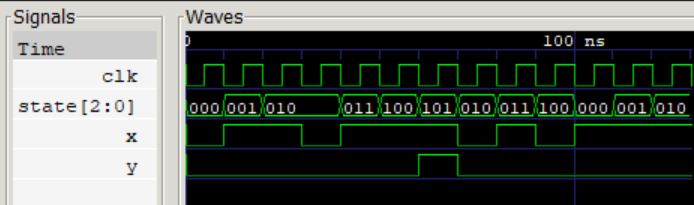
\includegraphics[width=1\linewidth]{figs/verilog.png}
    \caption{Moore Model}
    \label{fig:enter-label}
\end{figure}

\pagebreak

\begin{figure}
    \centering
    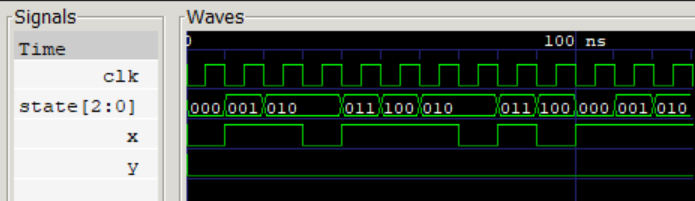
\includegraphics[width=1\linewidth]{figs/verilog1.png}
    \caption{Mely model}
    \label{fig:enter-label}
\end{figure}

\section{Results}
Images of circuits for some outputs,
\subsubsection{11011}
\begin{figure}[h!]
    \centering
    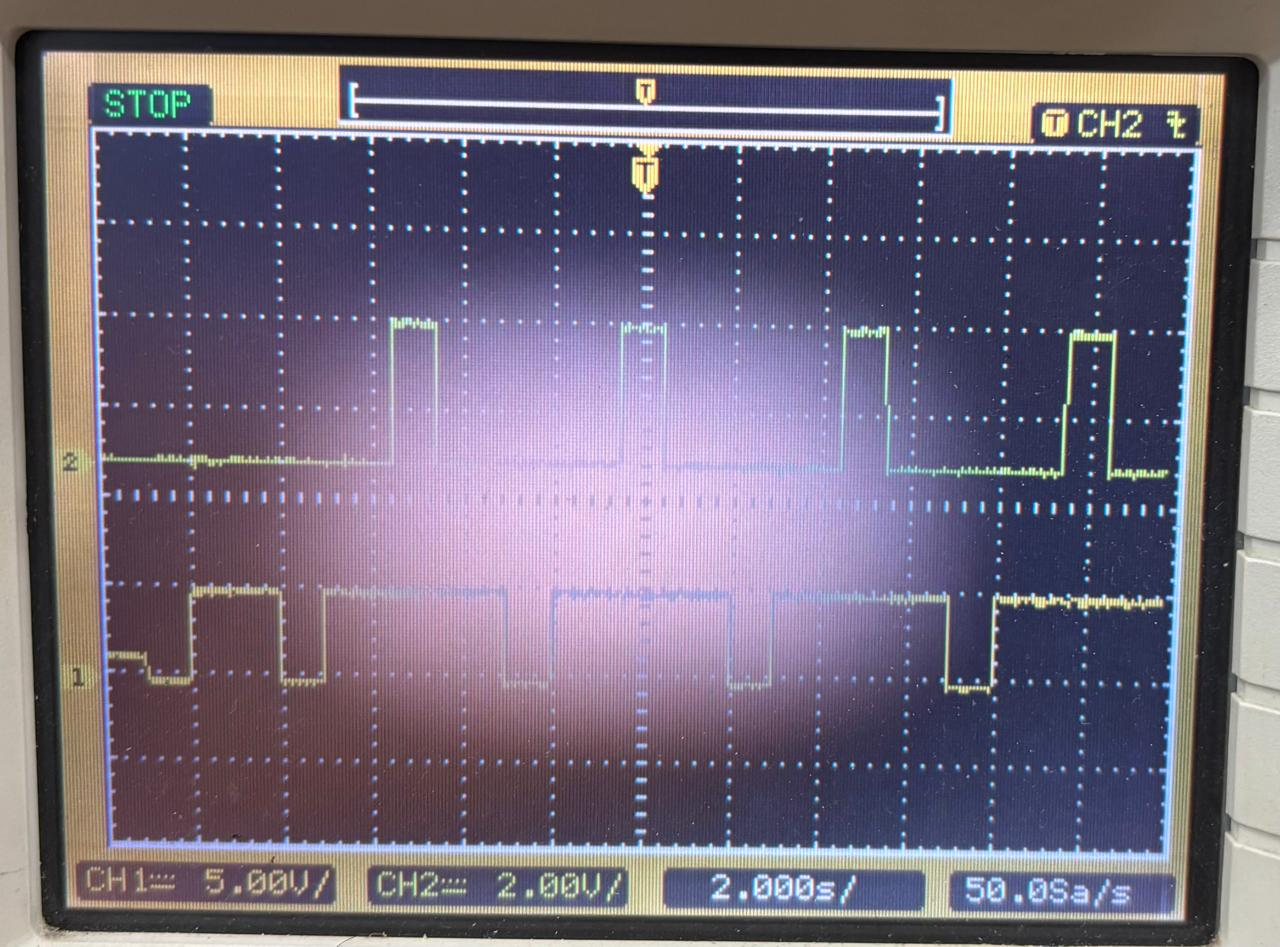
\includegraphics[width=0.7\linewidth]{figs/fig1.png}
    \label{fig:enter-label}
\end{figure}
\begin{figure}[h!]
    \centering
    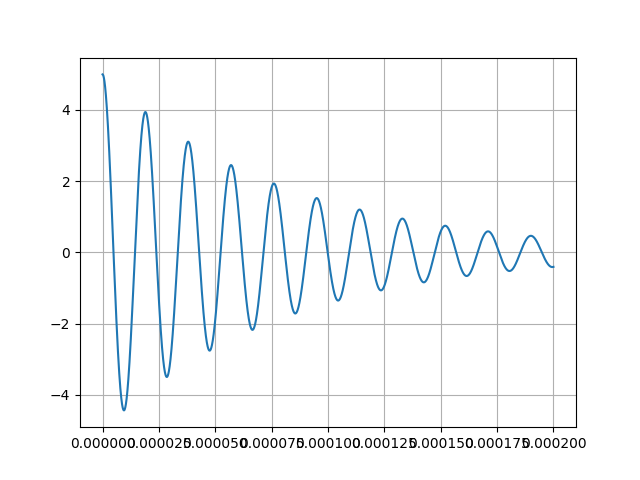
\includegraphics[width=0.5\linewidth]{figs/fig2.png}
    \label{fig:enter-label}
\end{figure}
\pagebreak
\subsubsection{1101110101}
\begin{figure}[h!]
    \centering
    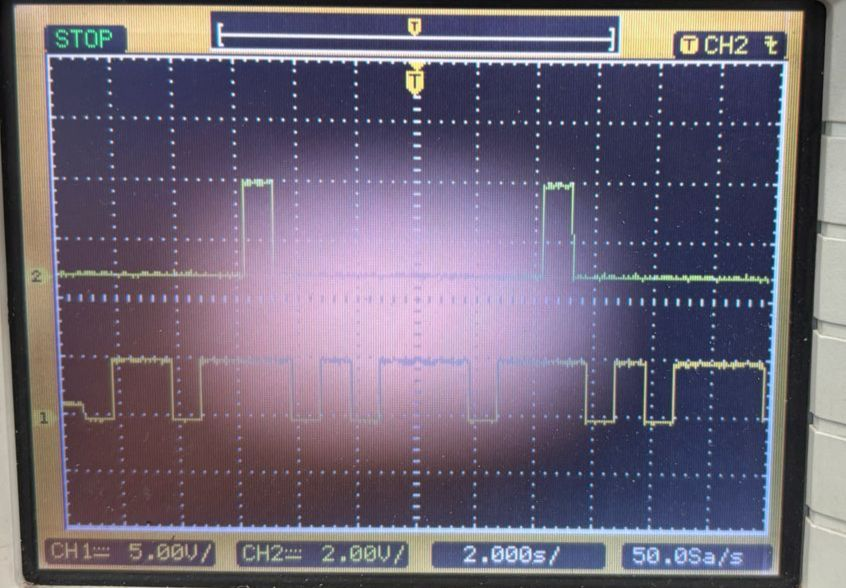
\includegraphics[width=0.7\linewidth]{figs/fig3.png}
    \label{fig:enter-label}
\end{figure}
\begin{figure}[h!]
    \centering
    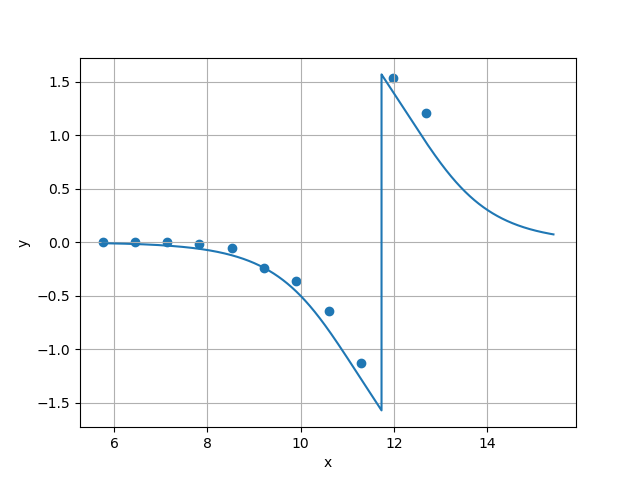
\includegraphics[width=0.6\linewidth]{figs/fig4.png}
    \label{fig:enter-label}
\end{figure}
\pagebreak
\subsubsection{0000011011}
\begin{figure}[h!]
    \centering
    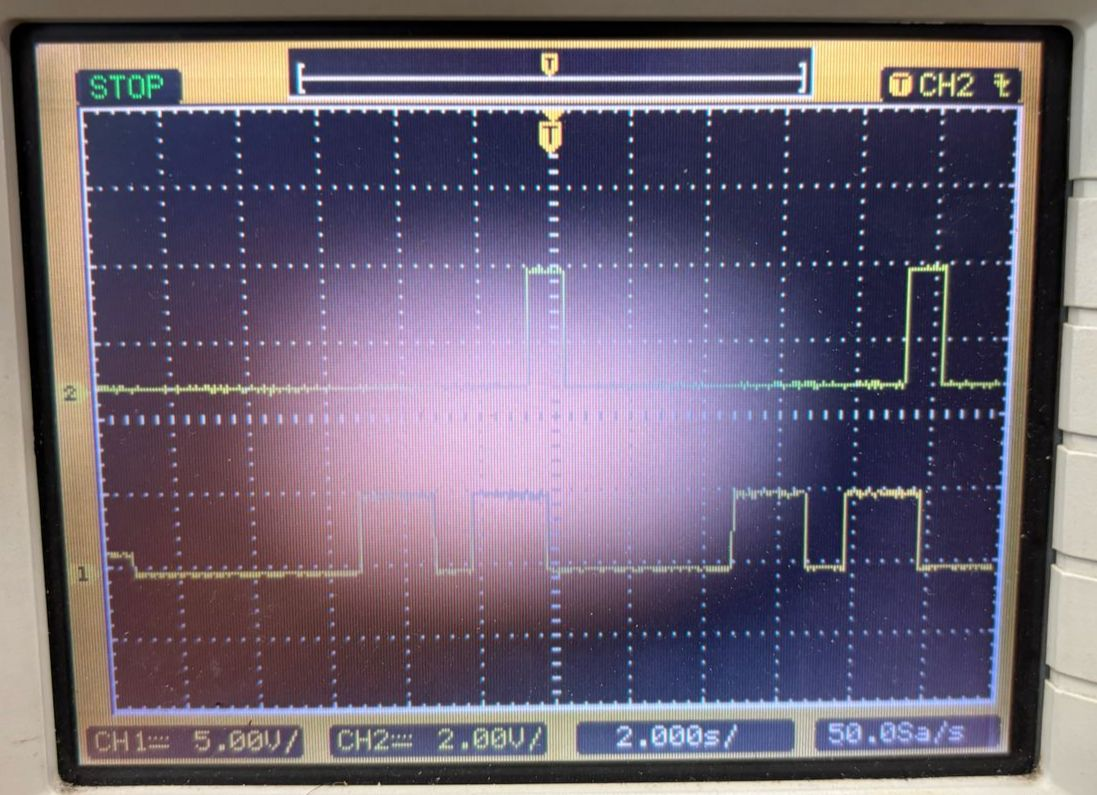
\includegraphics[width=0.7\linewidth]{figs/fig5.png}
    \label{fig:enter-label}
\end{figure}
\begin{figure}[h!]
    \centering
    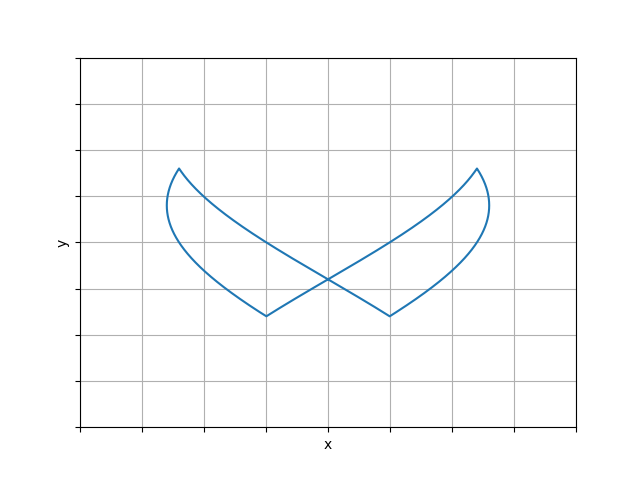
\includegraphics[width=0.6\linewidth]{figs/fig6.png}
    \label{fig:enter-label}
\end{figure}
\pagebreak
\subsubsection{0000011111}
\begin{figure}[h!]
    \centering
    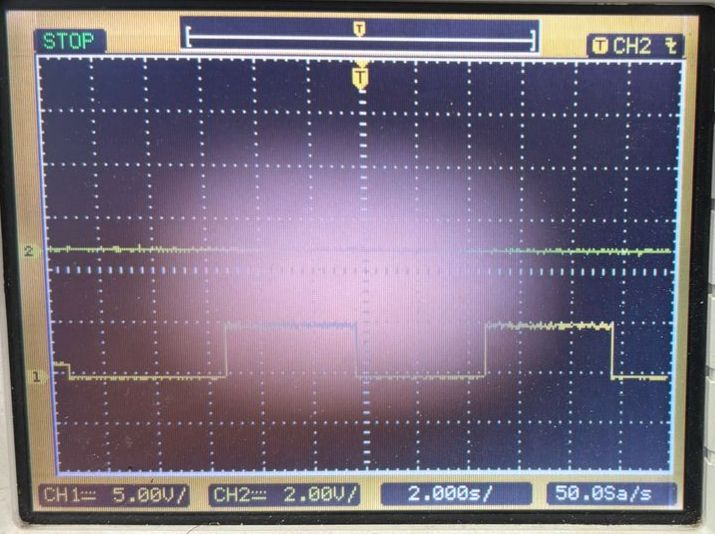
\includegraphics[width=0.7\linewidth]{figs/fig7.png}
    \label{fig:enter-label}
\end{figure}
\begin{figure}[h!]
    \centering
    \includegraphics[width=0.6\linewidth]{figs/fig8.png}
    \label{fig:enter-label}
\end{figure}
\pagebreak
\subsubsection{1101011011}
\begin{figure}[h!]
    \centering
    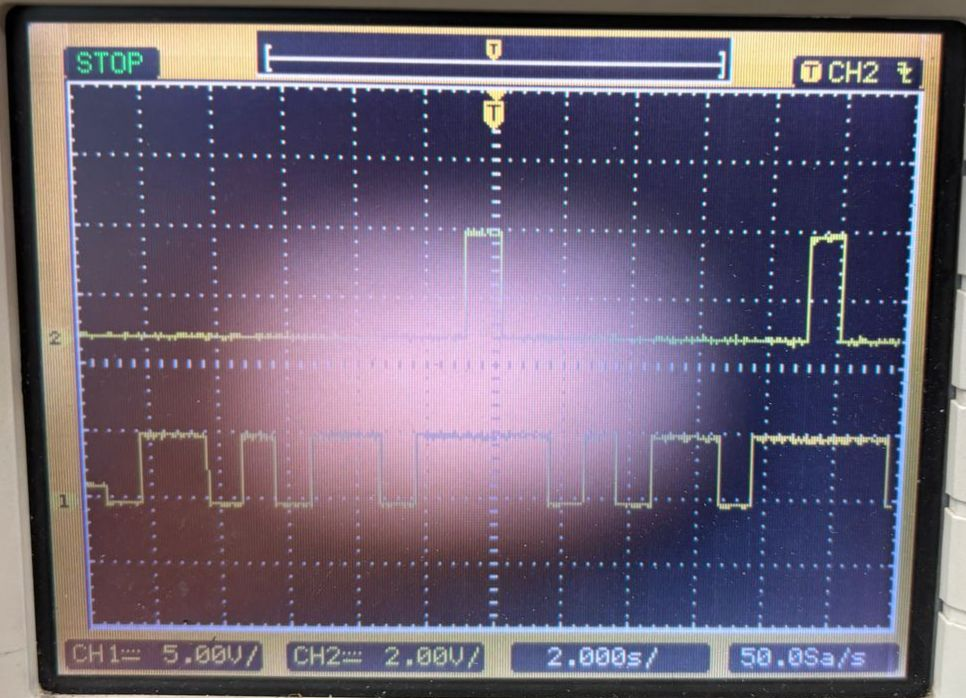
\includegraphics[width=0.7\linewidth]{figs/fig9.png}
    \label{fig:enter-label}
\end{figure}
\begin{figure}[h!]
    \centering
    \includegraphics[width=0.6\linewidth]{figs/fig10.png}
    \label{fig:enter-label}
\end{figure}
\pagebreak
\begin{align*}
&\text{Videos of working may be found here,}\\ &\text{\url{ https://github.com/ArjunPavanje/EE1200/tree/main/Experiment_9/vids}}
\end{align*}
\subsection{Why Moore over Mely?}
In case of a Mely counter there is no extra state (what we have defined as state-5 in our FSM). So, the output is read as $1$ (if it occurs) for a very short period of time only i.e. within the interval where transition from state-4 to either state-3 or state-2 happens in the negative edge of the clock. We can't observe the output properly in that case, so Moore counter is better as it has an extra state where output is $1$.  To conclude, in Mely counters,  in the same clock edge output becomes 1, and as soon as input signal is detected as $1$ and immediately becomes $0$ as it goes to state-$3$ or state-$2$, it is not particularly desirable as output is $1$ only for an extremely short period of time. One fix to this is to add a D-flip flop which allows the output to stay for one clock cycle. Another way is to implement a Moore counter as we have done.
\section{Conclusion}
This shows the building, and working of a moore machine which detects the sequence $11011$ in a given input signal using FSM (finite state machine).
\end{document}